\documentclass[border=5mm,tikz]{standalone}
\usepackage{pgfplots}
\usepgfplotslibrary{groupplots}
\pgfplotsset{compat=1.13}


\begin{document}
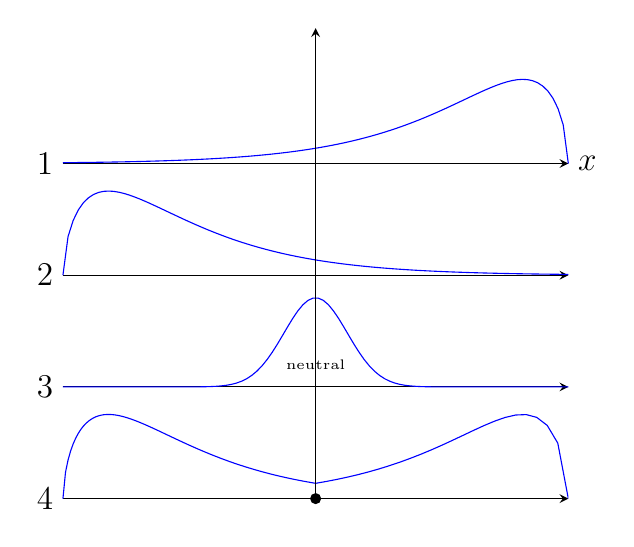
\begin{tikzpicture}[
declare function={
  gamma(\z) = 2.506628274631*sqrt(1/\z)+ 0.20888568*(1/\z)^(1.5)+ 0.00870357*(1/\z)^(2.5)- (174.2106599*(1/\z)^(3.5))/25920- (715.6423511*(1/\z)^(4.5))/1244160)*exp((-ln(1/\z)-1)*\z;},
    declare function={gammapdf(\x,\k,\theta) = 1/(\theta^\k)*1/(gamma(\k))*\x^(\k-1)*exp(-\x/\theta);},
    declare function={gauss(\x,\mu,\sig)=exp(-((\x-\mu)^2)/(2*\sig^2))/(\sig*sqrt(2*pi));}
]
\begin{groupplot}[
  group style={
    group size=1 by 4,
    vertical sep=0pt,
    group name=G},
  xtick=\empty,ytick=\empty,
  width=8cm,height=3cm,
  axis lines=middle,
  y axis line style={draw=none},
  ymax=0.5,
  clip=false,
  no markers,
  domain=0:8,
  samples=100]

\nextgroupplot[
    xlabel=$x$,
    x label style={right,font=\large,at={(rel axis cs:0,0)}},
    x axis line style={stealth-},
    x post scale=-1]
\addplot {gammapdf(x,1.6,1.2)};

\nextgroupplot
\addplot {gammapdf(x,1.6,1.2)};
\nextgroupplot
\addplot+ [domain=-8:8] {gauss(x,0,1)};
\node [font=\tiny] at (0,0.1) {neutral};
\nextgroupplot[xmin=0,xmax=8]
\addplot+ [domain=0:4] {gammapdf(x,1.6,1.2)};
\end{groupplot}

\begin{axis}[width=8cm,height=3cm,ymax=0.3,at={(G c1r4.south west)},x post scale=-1,hide axis,xmin=0,xmax=8,ymax=0.5,enlargelimits=false,no markers]
\addplot+ [domain=0:4] {gammapdf(x,1.6,1.2)};
\end{axis}


\node [left,font=\large] at (G c1r1.south west) {$1$};
\node [left,font=\large] at (G c1r2.south west) {$2$};
\node [left,font=\large] at (G c1r3.south west) {$3$};
\node [left,font=\large] at (G c1r4.south west) {$4$};

\draw [-stealth] (G c1r4.south) -- ([yshift=0.3cm]G c1r1.north);
\fill (G c1r4.south) circle[radius=2pt];
\end{tikzpicture}

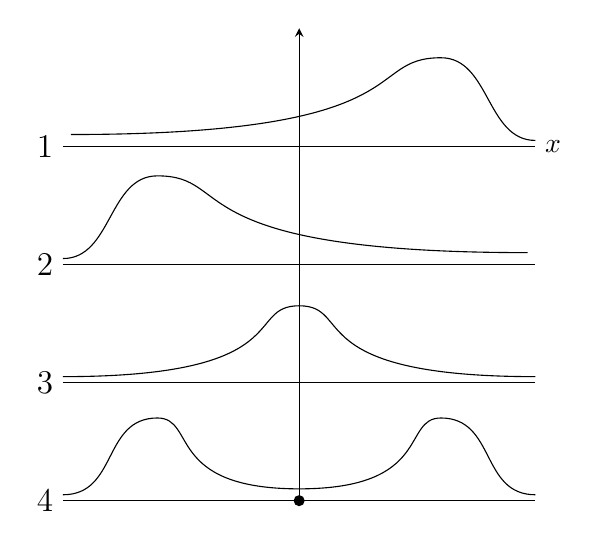
\begin{tikzpicture}[y=1.5cm]
\foreach [count=\i] \y in {4,3,2,1}
   \draw (0,\y) node [left,font=\large]{$\i$} -- (6,\y );
\node [right] at (6,4) {$x$};

\draw (0,3.05) to[out=0,in=180] ++(1.2,0.7) .. controls +(1,0) and  +(-4.5,0) .. ++(4.7,-0.65);
\draw (0,2.05) .. controls +(3,0) and  +(-0.7,0) .. (3,2.65) .. controls +(0.7,0) and +(-3,0) .. (6,2.05);
\draw (0,1.05) .. controls +(.7,0) and +(-.7,0)  .. (1.2,1.7) 
               .. controls +(0.5,0) and  +(-1.7,0) .. (3,1.1)
               .. controls +(1.7,0) and  +(-0.5,0) .. (4.8,1.7)
               .. controls +(0.7,0) and  +(-.7,0) .. (6,1.05);
\draw (6,4.05) to[out=180,in=0] ++(-1.2,0.7) .. controls +(-1,0) and  +(4.5,0) .. ++(-4.7,-0.65);

\fill (3,1) circle[radius=2pt];
\draw [-stealth] (3,1) -- (3,5);
\end{tikzpicture}
\end{document}